\documentclass[11pt]{article}
\usepackage{amsmath,amssymb,amsthm}
\usepackage{tabu}
\usepackage{graphicx}
%\usepackage[bw]{mcode}
\usepackage[margin=.6in]{geometry}
\usepackage{tikz}
\usepackage{float}
\usepackage{textcomp}
\usepackage{multicol}
\addtolength{\topmargin}{.5in}
\usepackage{fancyhdr}
\usetikzlibrary{positioning}
\usepackage{pgfplots}
\setlength{\parindent}{0pt}
\setlength{\parskip}{5pt plus 1pt}
\setlength{\headheight}{20pt}
\renewcommand{\headrulewidth}{0pt}
\setlength{\headheight}{30.0pt}
\newcommand\question[2]{\vspace{.25in}\hrule\textbf{#1: #2}\vspace{.5em}\hrule\vspace{.10in}}
\renewcommand\part[1]{\vspace{.10in}\textbf{(#1)}}
\newcommand\enter{\vspace{.50in}}
\newcommand\algorithm{\vspace{.10in}\textbf{Algorithm:}}
\newcommand\correctness{\vspace{.10in}\textbf{Correctness: }}
\newcommand\runtime{\vspace{.10in}\textbf{Running time: }}
\pagestyle{fancyplain}

\begin{document}\raggedright
\newcommand\Page{\page  / \lastPage}
\newcommand\page{1}
\newcommand\qN[2]{\Large {#1} \small{#2} \normalsize}

% info
\newcommand\dueDate{\today}
\newcommand\hwnum{3}
\newcommand\ExNum{}

\newcommand\lastPage{3}

% set info
\lhead{\large Homework \hwnum }
\rhead{\rightHead}
\chead{\LARGE{Root Finding Methods}}
\newcommand\rightHead{\large Due October 2, 2020}

\question{Submission}{}
Submissions should contain a single compressed folder (specifically .zip) that contains the following documents:
\begin{itemize}
	\item a single (typed) pdf document containing your answers to each question. Hand drawings are okay to upload.\\
	\item your .cpp files for each question\\
	\item name the folder Name\_HW\# where # indicates the homework \#\\
\end{itemize}

\vspace{5cm}
\question{1}{Root finding methods (10 pts)}
Explain the difference between a bracketing method and an open root finding method. List 2 examples of each method. 
\vspace{5cm}

\newpage
\question{2}{Bisection Method (15 pts)}
The Bisection method is a variation of the incremental search method in which the interval is always divided in half. If a function changes sign over the interval, the function at the midpoint is evaluated. The root is then determined to lie in the interval where the sign change occurs. That subinterval becomes the new interval for the next iteration. The process is repeated until the root is know to a required precision. 
\\\vspace{5pt}
Use this method to find the root of y(x)=2x-0.5. Iterate 5 times with your initial $a=0$, $b=2$. Draw your intervals on the figure below. Report $x_r$ and the percent relative error for each interval where applicable. Do not reference the pre-assessment for the first step or your answer will be wrong. 

\begin{figure}[H]
	\centering
	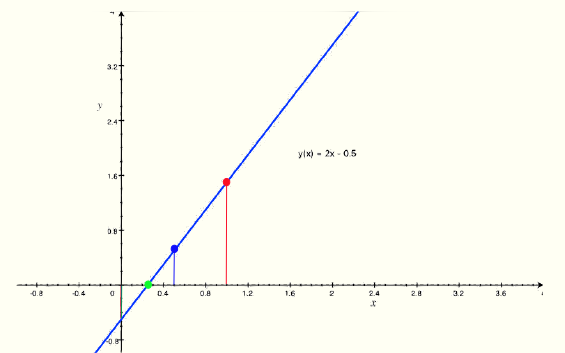
\includegraphics[width=0.8\textwidth]{plot}
\end{figure}
\vspace{2cm}
\textbf{iteration 1:}\\\vspace{2cm}
\textbf{iteration 2:}\\\vspace{2cm}
\textbf{iteration 3:}\\\vspace{2cm}
\textbf{iteration 4:}\\\vspace{2cm}
\textbf{iteration 5:}\\\vspace{2cm}

\question{3}{Bisection Method (15 pts)}
Modify the/submit your own bisection method code developed in lecture to determine the \textbf{drag coefficient, $c_d$,} needed so that an 95-kg bungee jumper has a velocity of 46 m/s after
9 s of free fall. Note: The acceleration of gravity is 9.81 m/s2.
Start with initial guesses of $x_l = 0.2$ and $x_u = 0.5$ and iterate
until the approximate relative error falls below 1\%. Report the value of $c_d$ and the number of iterations it took to find the root. \textbf{Submit your code.}

\newpage
\question{4}{Simple fixed-point iteration (15 pts)}
Open methods employ a formula to predict the root. Use simple fixed-point iteration to locate the root of $f(x)=\sin(\sqrt{x})-x$. Start with an initial guess of $x_0=0.5$ and iterate 6 times. Fill in the table below. 
\begin{table}[H]
	\centering
	\begin{tabular}{c | c | c}
		i & $x_i$ & $x_{i+1}$ \\
		\hline
		0 & 0.500000000 &  \qquad \qquad \qquad \qquad.\\ 
		\hline
		1 &  & \\
		\hline
		2 &	 & \\ 
		\hline
		3 &  & \\
		\hline
		4 &  & \\
 		\hline
 		5 &  & \\
	\end{tabular}
\end{table}
The root of this function is $\approx 0.7686488567609$. What do you notice about your results?\\
\vspace{4cm}



\question{5}{Newton-Raphson Method (15 pts)}
 Use the Newton-Raphson method to locate the root of $f(x)=\sin(\sqrt{x})-x$. Start with an initial guess of $x_0=0.5$ and iterate 6 times. Fill in the table below. Note: $f'(x) = \frac{1}{2\sqrt{x}}\cos(\sqrt{x}) -1$
\begin{table}[H]
	\centering
	\begin{tabular}{c | c | c}
		i & $x_i$ & $x_{i+1}$ \\
		\hline
		0 & 0.500000000 &  \qquad \qquad \qquad \qquad.\\ 
		\hline
		1 &  & \\
		\hline
		2 &	 & \\ 
		\hline
		3 &  & \\
		\hline
		4 &  & \\
		\hline
		5 &  & \\
	\end{tabular}
\end{table}
The root of this function is $\approx 0.7686488567609$. What do you notice about your results?\\

\newpage
\question{6}{Newton-Raphson Method (15 pts)}
Modify the/submit your own Newton-Raphson method code developed in lecture and apply it to the function $f(x) = \tanh(x^2-9)$ to evaluate its known real root at $x = 3$. Use an initial guess of $x_0 = 3.2$ and take a minimum of three iterations. \textbf{Submit your code.}\\
\vspace{6pt}
$\qquad x_1 =$ \\\vspace{6pt}
$\qquad x_2 =$ \\\vspace{6pt}
$\qquad x_3 =$ \\\vspace{6pt}

Did the method converge to its real root? \\\vspace{1cm}


Sketch the plot with the results for each iteration labeled.
\vspace{6cm}


\question{7}{Newton-Raphson Method (15 pts)}
Modify the/submit your own Newton-Raphson method code developed in lecture to determine the \textbf{drag coefficient, $c_d$,} needed
so that an 95-kg bungee jumper has a velocity of 46 m/s after
9 s of free fall. Note: The acceleration of gravity is 9.81 m/s2.
Start with initial guesses of $x_l = 0.2$ and $x_u = 0.5$ and iterate
until the approximate relative error falls below 1\%. Report the value of $c_d$ and the number of iterations it took to find the root. Compare your result to Question 3. \textbf{Submit your code.}

\end{document}
